\section{Proposed Research}

\subsection{Justification for Adopting a Bayesian Framework}

The Bayesian framework is not as computationally simple as the Frequentist framework.  Good justification is required for adopting a Bayesian perspective on Apixiban pharmacokinetics, especially in light of Frequentist non-linear mixed effect models for ODEs \cite{tornoe2004non}.  Here, I discuss just some benefits of adopting a Bayesian framework over a Frequentist framework.

In the proposed application, new patient's pharamcokinetic parameters will be estimated from the model with as few as one measurement per patient.  Estimating several parameters from a single observation in a mixed effects model presents statistical obstacles which are difficult to overcome.  In a Bayesian framework, the prior distribution can make estimating these parameters from sparse data possible.  Of course, this relies on an informative prior.  However, my partnership with clinical pharmacologists will provide rich pharmacological experience to the project, which can then be translated into appropriate and informative priors.  Moreover, the asymptotic arguments used to develop tests of hypothesis in Frequentism may not be valid in application because sample sizes are so small.  Adopting a Bayesian framework will allow for explicit modelling of uncertainty propagation without assuming that asymptotics are valid.

Finally, sequential decision making plays a central role in the proposed research \'{a} la reinforcement learning.  Since posteriors from previous experiments can be used as priors for future experiments, Bayesianism provides a natural framework for sequential evaluation of evidence and decision support.


\subsection{Bayesian Pharmacokinetic Models}

The construction of appropriate Bayesian models for application is non-trivial.  Great care should be taken to construct a model which is sufficiently complex to capture relevant features of the phenomenon, but not so complex as to over fit on the data. 

 The line between appropriately complex and overfit models is not easy to discern.  A recommended strategy for constructing Bayesian models is to start simple, essentially from a model which is ostensibly wrong, and slowly build in complexity, checking the model's implications and improving the model where needed.  Gelman calls this process ``continuous model expansion" \cite{gelman2013bayesian, gelman2013philosophy}.  For the proposed research, a very simple Bayesian model of Apixiban pharmacokinetics will be proposed.  Several expanded models will also be considered and further expanded where needed. Models will be assessed by checking for patterns in the residuals as well as posterior predictive checks.

Data from a controlled experiment \cite{tirona2018apixaban} will be used as a ``development set''.  The data contain 36 patients observed over 12 hours. Each subject ingested 2.5 mg of Apixiban and 100 ml of water in a fasted state. Apixiban blood plasma concentrations were recorded, as well as subject covariates.  See \cref{devsettable} for a summary of patients involved.

\begin{table}[b!]
	\centering
\begin{tabular}{lrrrr}
	\toprule
	\multicolumn{1}{c}{ } & \multicolumn{2}{c}{Female} & \multicolumn{2}{c}{Male} \\
	\cmidrule(l{2pt}r{2pt}){2-3} \cmidrule(l{2pt}r{2pt}){4-5}
	& \multicolumn{1}{c}{Control } & \multicolumn{1}{c}{ NAFLD}  & \multicolumn{1}{c}{ Control}  & \multicolumn{1}{c}{NAFLD } \\
	\midrule
	N & 10 & 13 & 2 & 11\\
	Age  & 46.40 (9.13) & 50.62 (13.24) & 57.00 (18.38) & 50.73 (10.96)\\
	Weight (kg)& 85.77 (27.70) & 83.76 (20.93) & 74.60 (17.82) & 97.56 (25.74)\\
	Creatinine ($\mu$M)& 65.70 (10.34) & 70.62 (13.36) & 86.50 (12.02) & 63.73 (10.76)\\
	\bottomrule
\end{tabular}

\caption[Summary of development data set]{Covariate summary for patients in development set \cite{tirona2018apixaban}.  Shown are sample means with sample standard deviations in parentheses.  Data is stratified by sex and group status (patients with and without non-alcoholic fatty liver disease (NAFLD)).}
\label{devsettable}

\end{table}

\begin{figure}[t!]
	\centering
	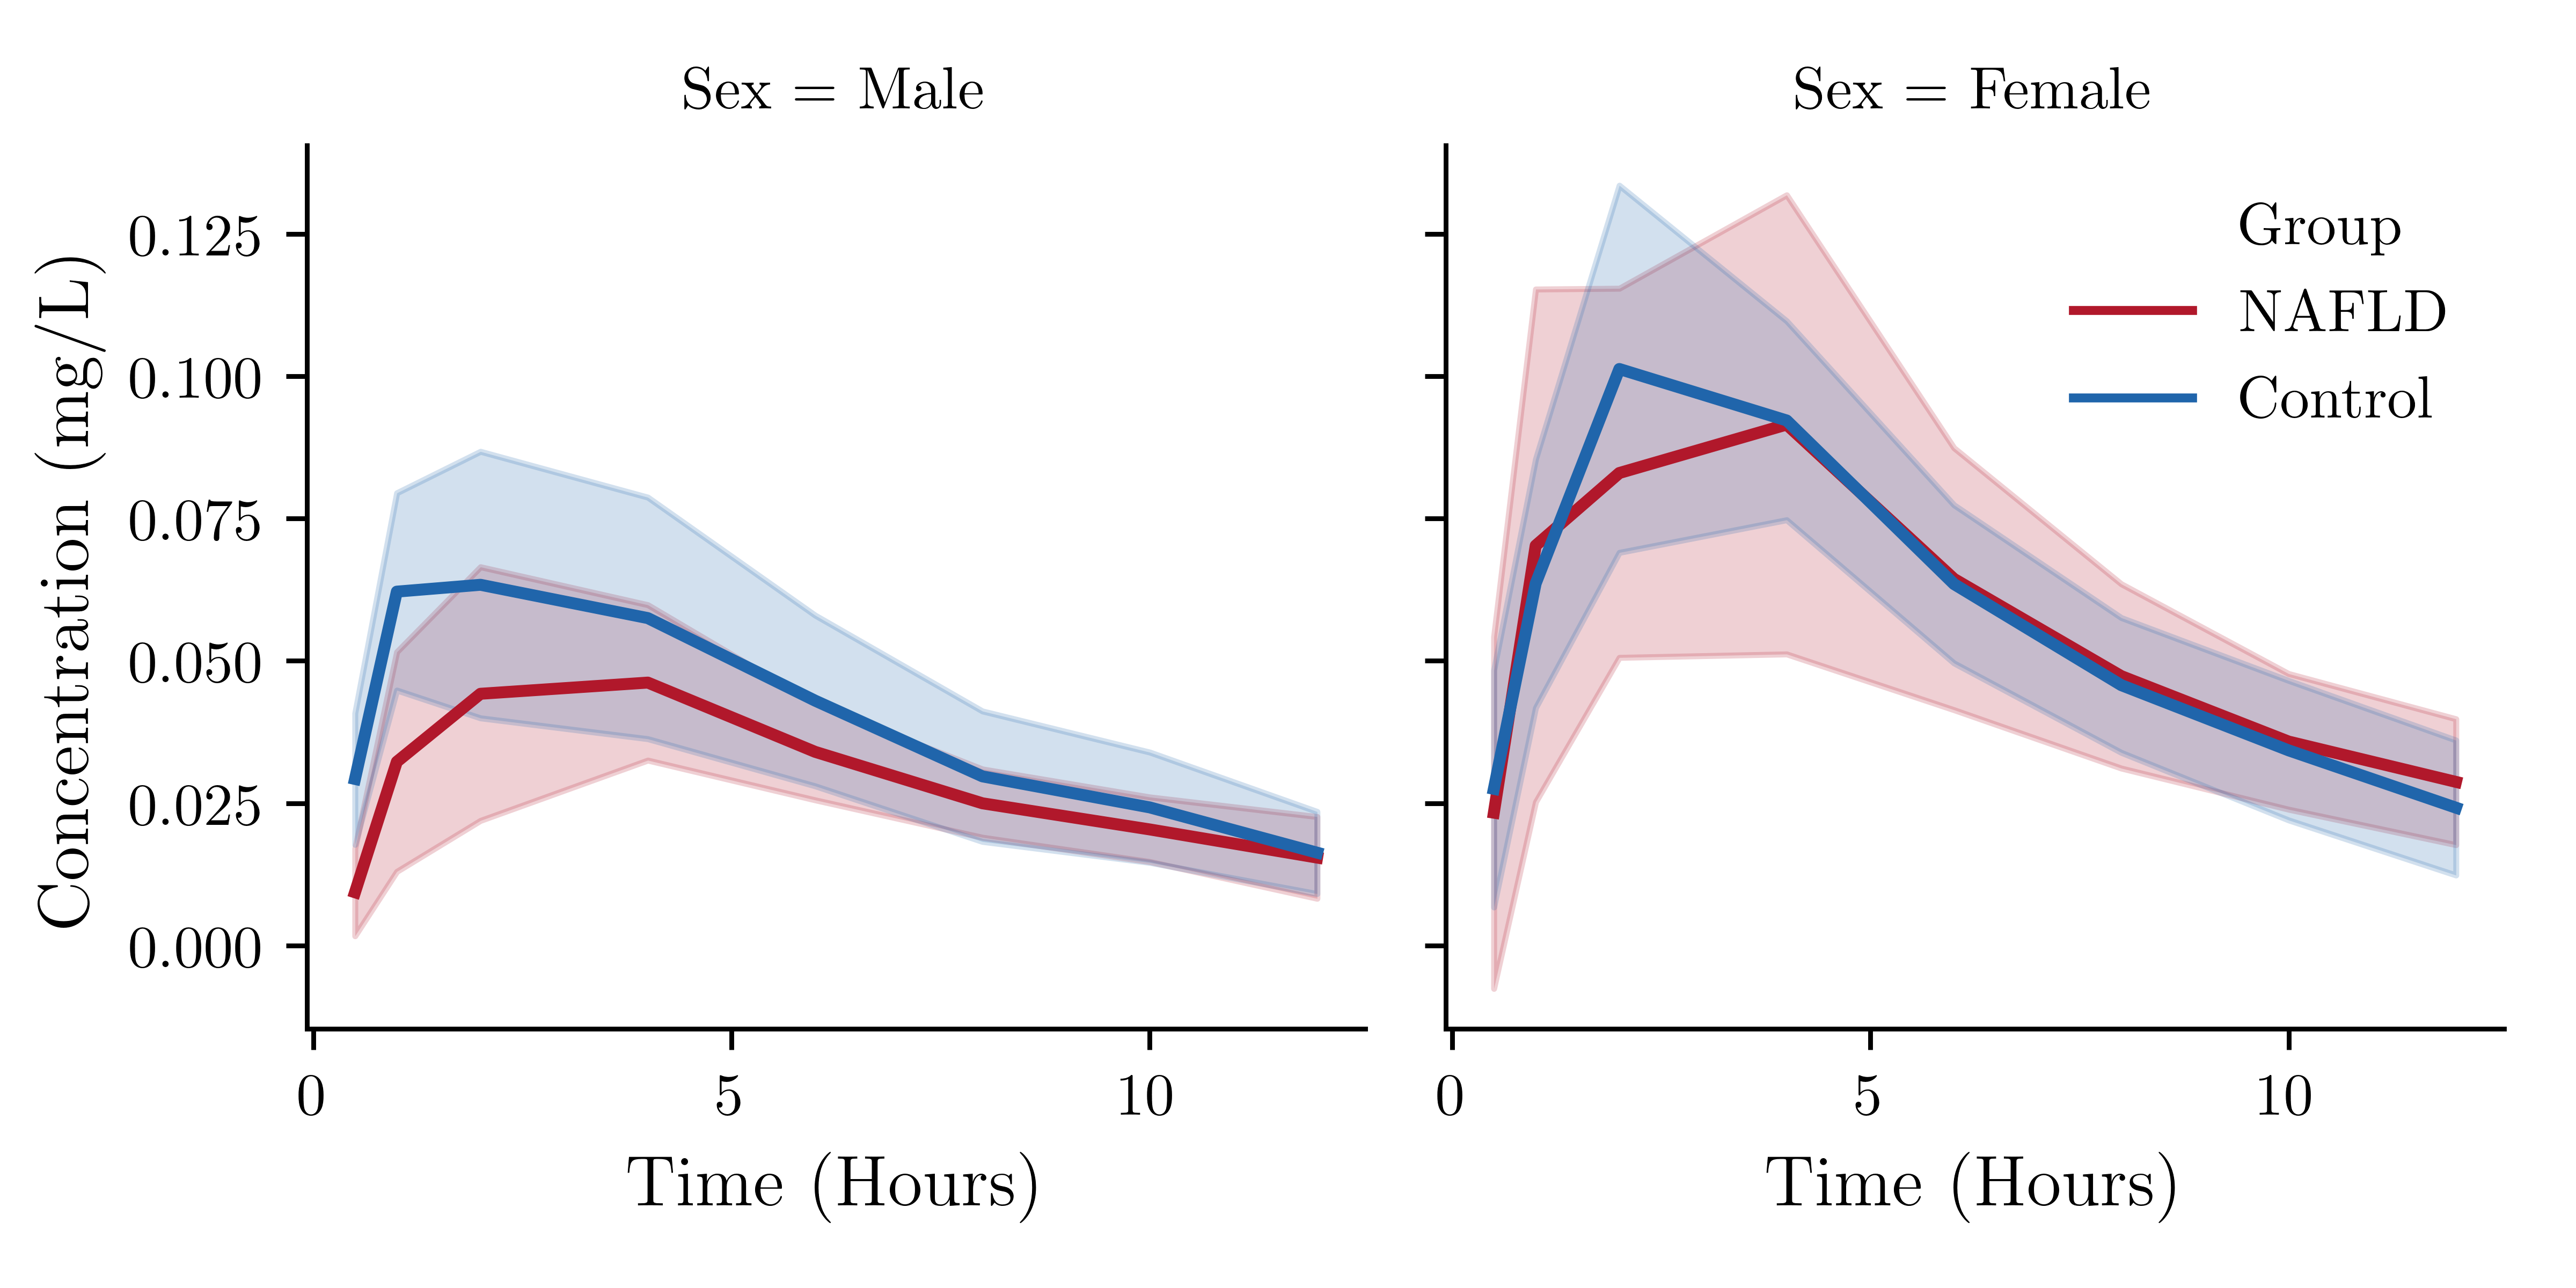
\includegraphics{Figures/data_summary}
	\caption[Concentration profiles for development set]{Concentration profiles for each group of the development set.  Colors indicate group, shaded regions indicate one standard deviation.  There appears to be a noticeable effect of sex on concentration.}
	\label{datasummary}
\end{figure}







\subsection{Adaptive Sampling}

\subsection{Adaptive Control}
